\documentclass{article}%
\usepackage[T1]{fontenc}%
\usepackage[utf8]{inputenc}%
\usepackage{lmodern}%
\usepackage{textcomp}%
\usepackage{lastpage}%
\usepackage{authblk}%
\usepackage{graphicx}%
%
\title{Baicalein Reduces the Invasion of Glioma Cells via Reducing the Activity of p38 Signaling Pathway}%
\author{Cheryl Ramirez}%
\affil{Blood Transfusion Centre of Slovenia, Ljubljana, Slovenia}%
\date{01{-}01{-}2013}%
%
\begin{document}%
\normalsize%
\maketitle%
\section{Abstract}%
\label{sec:Abstract}%
C{-}KIT MARKER CHK 1, which was taken from the cells of a heart, was elevated to within 200 nm from 250 nm and is recognized as an extracellular marker, a kind of bedside{-}home indicator that indicates the fate of a cardiac cell. Nearly 2600 individuals with coronary artery disease had c{-}kit markers within 2000 nm of heart cell death as measured by the patients ventricular perfusion test during clinical hospitalization. In summary, patient cardiac cells were found to be grossly overexpressed and highly polarized, but the critical parameter of c{-}kit signaling appeared to have fully returned to normal levels.\newline%
Nemesis the cardiologist: a doubling in cardiac cells was observed shortly after cardiac transplantation and 32\% fewer cells were found within 2\% of extracellular markers. Based on his research, Herv Aeder, MD, of the University Hospital of San Diego in La Jolla and colleagues turned to a self{-}healing substance which could lead to more efficient methods of improving cardiac cell health. They took the active ingredient dextromethorphan and added it to the mixture of varlosone and epigallocatechin gallate. Increased cardiac cell overexpression was observed in a number of cardiac cell lines in vitro. In immunodeficient mice, epigallocatechin gallate boosted the expression of c{-}kit signaling while removing cytokines, which inhibited the natural signaling process. Researchers showed a marked survival of the fittest effect in the laboratory. Within 8 hours of exposure to epigallocatechin, the gene coding for c{-}kit gene expression had returned to normal levels.\newline%
 This study can greatly improve future development and application of therapeutic diagnostic tests. It is shown that certain cardiac therapies could be tailored to our individual conditions and that this test could be customized to focus on therapeutic agents.\newline%
April 2013

%
\subsection{Image Analysis}%
\label{subsec:ImageAnalysis}%


\begin{figure}[h!]%
\centering%
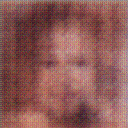
\includegraphics[width=150px]{500_fake_images/samples_5_494.png}%
\caption{A Black And White Photo Of A Black And White Photo}%
\end{figure}

%
\end{document}